\documentclass[12pt,letterpaper]{article}

\usepackage{amsmath} 
\usepackage{amssymb}
\usepackage{ulem}
\usepackage{tikz}
\usepackage[left=1in,top=1in,right=1in,bottom=1in,nohead]{geometry}
\usetikzlibrary{decorations.markings}
\usetikzlibrary{decorations.pathreplacing}

\usepackage{amsthm} 
\usepackage{wrapfig}
\usepackage{enumitem}
%\usepackage{enumerate}
\newtheorem{mydef}{Definition}
\newtheorem{example}{Example}
\newtheorem{thrm}{Theorem}
\newtheorem{lemma}{Lemma}
\newtheorem{cor}{Corollary}
\newtheorem{notation}{Notation}
\newtheorem{rem}{Remarks}
\newcommand{\biu}[1]{\underline{\textbf{\textit{#1}}}}
\newcommand{\so}{\Rightarrow}
\usepackage[ampersand]{easylist}

\let\oldemptyset\emptyset
\let\emptyset\varnothing

\newcommand{\homework}{\biu{Homework}}
\newcommand{\Mor}{\text{Mor}}
\newcommand{\N}{\mathbb{N}}
\newcommand{\Q}{\mathbb{Q}}
\newcommand{\Z}{\mathbb{Z}}
\newcommand{\R}{\mathbb{R}}
\newcommand{\C}{\mathbb{C}}
\newcommand{\pabs}[1]{\left|\left| #1 \right|\right|_p}
%\newcommand{\pabs}[1]{#1}
\begin{document}
\tikzstyle{lattice}=[shape=circle,draw,fill,text=white]
\tikzset{
  % style to apply some styles to each segment of a path
  on each segment/.style={
    decorate,
    decoration={
      show path construction,
      moveto code={},
      lineto code={
        \path [#1]
        (\tikzinputsegmentfirst) -- (\tikzinputsegmentlast);
      },
      curveto code={
        \path [#1] (\tikzinputsegmentfirst)
        .. controls
        (\tikzinputsegmentsupporta) and (\tikzinputsegmentsupportb)
        ..
        (\tikzinputsegmentlast);
      },
      closepath code={
        \path [#1]
        (\tikzinputsegmentfirst) -- (\tikzinputsegmentlast);
      },
    },
  },
  % style to add an arrow in the middle of a path
  end arrow/.style={postaction={decorate,decoration={
        markings,
        mark=at position 1 with {\arrow[#1]{stealth}}
      }}},
}

Suppose $(X,d)$ is a metric space and $(x_n)_{n\geq 1}$ a sequence in $X$.
\begin{mydef}
$(x_n)$ is a Cauchy sequence if, for each $\epsilon > 0$, there exists $N$ such that $m,n\geq N\so d(x_n,x_m)<\epsilon$.
\end{mydef}
\begin{rem}
Every convergent sequence is Cauchy:
\begin{proof}
Suppose $\lim x_n\to x_\infty$ exists. Then $d(x_n,x_m)\leq d(x_n,x_\infty) + d(x_m,x_\infty)<2\epsilon$ if $N$ is subject to the condition $n>N\so d(x_n,x_\infty) < \epsilon$
\end{proof}
\end{rem}
\begin{mydef}
The metric space is complete if every Cauchy sequence coverges.
\end{mydef}
\begin{example}
\begin{enumerate}
\item $\R$ with its usual metric is complete
\begin{proof}
\homework
\end{proof}
\item $\Q$ is not complete
\item $\R^n$ with the euclidean distance metric is complete \par
We shall proof this assertion using a series of definitions and observations that will also be otherwise useful. \par
\end{enumerate}
\end{example}
Suppose $d_1,d_2$ are two distance functions on a set $X$.
\begin{mydef}
$d_1$ and $d_2$ are mutually bounded if $\exists$ constants $c>0$, $D>0$, such that $cd_1(x,y)\leq d_2(x,y) \leq Dd_1(x,y) \forall x,y\in X$. Note that this is an equivalence relation.
\end{mydef}
\begin{obs}
Any two mutually bounded metrics determine the same notions of convergence of Cauchy sequences. 
\end{obs}
Suppose $(X_i,d_i)_{1\leq i\leq N}$ are metric spaces (with all $X_i \neq \emptyset$. Define the product metric on the Cartesian product $\prod\limits_{i=1}^N X_i$ by $d(x,y)=\sum\limits_{i=1}^N d(x_i,y_i)$. Note that this function satisfies all the properties fir a metric.
\begin{obs}
$(X,d)$ is complete if and only if each $(X_i,d_i)$ is complete. 
\begin{proof}
A sequence $(x^n)_{n \geq 1}$ in $X$ converge, is Cauchy iff each of the component sequence $(x_i^n)_{m\geq 1}^{1\leq i\leq N}$ converge, resp. is Cauchy. 
\end{proof}
\end{obs}
Let $d_{st}$ be the standard (euclidean) distance on $\R^k$, $d_{prod}$ the product distance. For $x,y\in\R^k$
\begin{align} 
|x_i-y_i| &\leq& \sqrt{\sum\limits_{j=0}^N (x_j-y_j)^2} &\leq& \sum\limits_{j=0}^N |x_j-y_j| \\
\so \frac{1}{k}d_{prod}(x,y)&\leq& d_{st}(x,y)&\leq& d_{prod}(x,y)
\end{align}
This proves that $\R^k$ (with either the euclidean or the product metric) is complete because $\R$ is complete.
\section*{Open/Close/Dense Sets}
Suppose we have a metric space $(X,d)$ and some element $x_0 \in X$ of that metric space
\begin{mydef}
For $\epsilon > 0$, let $B(x_0,\epsilon)$ be the (open) ball centered at $x_0$ with points given by:
\[ x_0 =_{def} \{x\in X | d(x,x_0)<\epsilon \} \]
\end{mydef}
\begin{mydef}
 A subset $U\subset X$ is open if, for each $x_0\in U$, there exists $\delta>0$, s.t. $B(x_0,\delta)\subset U$. $S\subset X$ is closed if $X-S$ is open.
\end{mydef}
\begin{obs}
Arbitrary unions and finite intersections of open sets are open. Finite unions and a arbitrary intersections of closed sets are closed. $X$ and $\emptyset$ are both open and closed.
\begin{proof}
For the first statement note that we must have
\[ \bigcup_j B(x_0,\delta_j) \supset B(x_0,\delta_k) \]
i.e since all the sets over which the union is taken are open there must be at least one ball in the union of all balls centered at a particular point $x_0$ (namely a ball that also existed in one of the original sets). \par
A similar observation can be made for finite intersections:
\[ \bigcap_{i=0}{n} B(x_0,\delta_j) = B(x_0, min \delta_j) \]
i.e. the smallest of all balls centered at $x_0$ in one of the original sets must still exists. Note that the restriction that the intersection be finite stems from the fact that that in the limit the smallest $\delta_k$ could go to zero, which would not be allowed. \par
Furthermore note that the first and second sentence in the original observation are equivalent (they are complements of each other). And thus we are done.
\end{proof}
\end{obs}
\begin{mydef}
For $S \subset X$, the closure of $S$ is the smallest closed subset of $X$ which contains S. \par 
\end{mydef}
Note that the closure and interior exists as they be defined as 
\[ clos(S) = \bigcap_{\substack{T\subset X_{closed} \\ T \supset S}} T \]
\[ int(U) = \bigcup_{\substack{O\subset X_{open} \\ O \subset U}} O \]
\begin{thrm}
\begin{enumerate}
\item A subset $S\subset X$ is closed if and only if for every sequence $(x_n)$ which converges in $X$, S contains the limit $\lim\limits_{n\to\infty} x_n$.
\item $clos(S)=\{ \lim\limits_{n\to\infty} x_n | (x_n)$ sequences in $S$ converging in $X\}$
\end{enumerate}
\end{thrm}
\biu{Caution:} Both statements are not necessarily true in arbitrary topological spaces.
\begin{proof}
\begin{enumerate}
\item \biu{"if":} Suppose every sequence $(x_n)$ in $S$ which converges in $X$ has its limit in $S$, but $S$ is not closed. Then $X-S$ is not open. Therefore, there exists $x_0\in X$ such that $B(x_0,\frac{1}{n}) \not\subset X-S$ for all $n$.
\[ \so B(x_0,\frac{1}{n}) \cap S \neq \emptyset \so \exists x_n\in S, x_n \in B(x_0,\frac{1}{n}) \]
Then $x_n$ is a sequence in $S$, such that $d(x_n,x_0)<\frac{1}{n}$ so $\lim\limits_{n\to\infty} x_n = x_0$. So $(x_n)$ is a sequence in $S$ which converges to a point not in $S$ \biu{Contradiction}
\par\biu{"only if":} Suppose $S$ is closed but there exists a sequence $(x_n)$ in $S$ which converges to some $x_0\notin S$. $X-S$ is open so $\exists \epsilon>0$ s.t. $B(x_0,\epsilon)\subset X-S$. Then $B(x_0,\epsilon) \cap S$, but for $n \geq N$, $d(x_n,x_0)<\epsilon$, so $x_n$ does lie in both $B(x_0,\epsilon)$ and $S$. \biu{Contradiction}.
\item \par Given $x \in S$, the limit of the sequence $(x,x,x,\ldots)$ is $s$ so $S\subset\bar{S}=\{\lim\limits_{n\to\infty} x_n | (x_n)$ is a sequence in $S$, converging in $X\}$ \par 
To show that $\bar{S}$ is closed we will use 1): We shall show that every sequence $(\bar{x_n})$ in $\bar{S}$ which converges in X has a limit in $\bar{S}$. Each $\bar{x_n}\in\bar{S}$, hence is the limit of some sequence in S.
\[ \so \exists x_n \in S, d(x_n,\bar{x_n})<\frac{1}{n} \]
Then with $\bar{x} = \lim\limits_{n\to\infty} \bar{x_n}$
\[ d(x_n,\bar{x} \leq d(x_n,\bar{x_n}) + d(\bar{x_n},\bar{x}) < d(\bar{x_n},\bar{x}) + \frac{1}{n} \]
So, choosing $N$ sufficiently large, for $n\geq N$, 
\[d(\bar{x_n},\bar{x})<\epsilon,\frac{1}{n}<\epsilon \so d(\bar{x_n},\bar{x}) < 2\epsilon \]
so $\bar{x}=\lim\limits_{n\to\infty} x_n \so \bar{x}\in\bar{S}$. \par 
So $\bar{S}$ is closed and $S\subset \bar{X}, T closed$. To show that $\bar{S}$ is the closure of $S$, we need to show that $\bar{S}\subset T$, which is true by $1)$.
\end{enumerate}
\end{proof}
\section{Isometry}
Suppose $(X_i,d_i)$, $i=1,2$ are metric spaces.
\begin{mydef}
$F: X_1 \to X_2$ is an isometry if $d_2(F(x'),F(x''))=d_1(x',x'')$. Any isometry is necessarily injective.
\end{mydef}
\begin{mydef}
$S\subset X$ is dense in $X$ if $clos(S)=X$
\end{mydef}
\begin{mydef}
Let $(X,d)$ be a metric space. A completion of $(X,d)$ is a metric space $(\bar{X},\bar{d})$ s.t. $X\subset d=\bar{d}|_x$, s.t. $(\bar{X},\bar{d})$ is complete with $X$ dense in $\bar{X}$.
\end{mydef}
\begin{thrm}
The completion exists and is unique in the following sense: if there exist completions $(\bar{X},\bar{d})$, $(\tilde{X},\tilde{d})$, then there exists a unique bijection $F: \bar{X}\to\tilde{X}$, which also is an isometry: \par
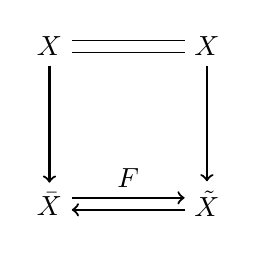
\begin{tikzpicture}[node distance=2cm, auto]
  \node (X) {$X$};
  \node (X2) [right of=X] {$X$};
  \node (Xb) [below of=X]{$\bar{X}$};
  \node (Xt) [below of=X2]{$\tilde{X}$};
  \draw [->,thick] (X) -- (Xb);
  \draw [->,thick] (X2) -- (Xt);
  \draw (X.15) -- (X2.165) (X.-15) -- (X2.195);
  \draw [->,thick] (Xb.15) to node {$F$} (Xt.165);
  \draw [->,thick] (Xt.195) -- (Xb.-15);
\end{tikzpicture}
Suppose $X$ is a set, $\sim$ an equivalence relation on $x$. An equivalence class for $\sim$ is a subset of $X$ of the following type:
\[ \{ x\in X|x\sim x_0\} \]
which is the equivalence class of $x_0$.
For all $x_0, x_1\in X$, the equivalence class of $x_0$ and the equivalence class of $x_1$ either
\begin{enumerate}
\item coincide
\item are disjoint
\end{enumerate}
\end{thrm}
$X/\sim$ is the set of equivalence classes. \par
Let $x\neq \emptyset, d: X\times X\to\R_{\geq 0}$ where $d$ is a function which satisfies a,, the requirements except that $d(x,y) = 0$ need not imply $x=y$. Then $d$ is called a pseudometric. Define a relation $\sim$ on $X$, $x\sim y \iff d(x,y)=0$.
\begin{lemma}
This is an equivalence relation.
\begin{proof}
Suppose $x\sim y$, $y\sim z$. Then $0\leq d(x,y) \leq d(x,y) + d(y,z)  = 0$
\end{proof} 
\end{lemma}
\begin{mydef} $\tilde{X}=X/\sim$ \end{mydef}
\begin{lemma} For $x,y\in X$, $d(x,y)$ depends only on the equivalence classes of $x,y$
\begin{proof}
Suppose $x_1 \sim x_2$. $d(x_1,y)\leq d(x_1,x_2) + d(x_2,y) = d(x_2,y)$. 
By symmetry we find $d(x_1,y) = d(x_2,y)$.
\end{proof}\end{lemma}
We can therefore define $\tilde{d}: \tilde{X}\times\tilde{X}\to\R_{\geq 0}$ as $\tilde{d}(\tilde{x},\tilde{y}) = d(x,y)$ if $x\in \tilde{x}$, $y\in \tilde{y}$.
\begin{lemma}
$(\tilde{X},\tilde{d})$ is a metric space
\begin{proof}
We only need to show that $\tilde{d}(\tilde{x},\tilde{y})=0 \so \tilde{x} = \tilde{y}$ (since all other properties hold for $d$, they must hold for $\tilde{d}$ as well). This is true however, by the definition of $\tilde{d}$
\end{proof}
\end{lemma}
Define $X^*=\text{set of all cauchy sequences in } X$.
\begin{lemma}
For $(x_n),(y_n)\in X^*$, $d(x_n,y_n)$ is a Cauchy sequence in $\R$,
\begin{proof}
\[ d(x_m,y_m)\leq d(x_m, x_n) + d(x_n,y_n) + d(y_n,y_m) \]
\[ \so d(x_m,y_n) - d(x_n,y_n) \leq d(x_m,x_n)  + d(y_n,y_m) \]
By using symmetry in $n,m$ we find
\[ |d(x_m,y_m)-d(x_n,y_n)| \leq d(x_n,x_m) + d(y_n,y_m) \]
The RHS can vbe made $<\epsilon$ is $m,n\geq N(\epsilon)$, $\so \lim\limits_{n\to\infty}$ exists in $\R_{\geq 0}$, and, because $\R$ is complete, $\R_{\geq 0}\subset R$ is closed.
\end{proof}
\end{lemma}
\begin{mydef}
$d^*: X*\times X*\to\R_{\geq 0}, d^*((x_n),(y_n))=\lim\limits_{n\to\infty} d(x_n,y_n)$
\end{mydef}
\begin{claim}
$(X^*,d^*)$ is a pseudometric space.
\begin{proof}
Clearly
\begin{eqnarray*}
d^*((x_n),(x_n)) = 0\\
d^*((x_n),(y_n)) = d^*((y_n),(x_n)) \\
d^*((x_n),(z_n)) \leq d^*((x_n),(y_n))+d((y_n),(z_n))
\end{eqnarray*}
All of the above are true term-by-term, hence they must be true in the limit (note that the third statement holds because, for any three convergent sequences of real numbers $(a_n),(b_n),(c_n)$
\[ a_n\leq b_n + c_n \so \lim\limits_{n\to\infty} a_n \leq \limn b_n + \limn c_n \]
). 
\end{proof}
\end{claim}
\begin{mydef}
$\bar{X}=X^*/\sim$, $\bar{d}$ is the metric on $\bar{X}$ induced by the pseudometric $d^*$ on $X^*$.
\end{mydef}
Then by earlier discussion $(\bar{X},\bar{d})$ is a metric space.
\begin{mydef}
$i: X \to \bar{X}$, $i(x) = $ equivalence class of the constant sequence $(x,x,x,\ldots)$
\end{mydef}
We have $\bar{d}(i(x),i(t))=[\limn$ all constant sequence $d(x,y)] = d(x,y)$. Therefore, $i:X\to\bar{X}$ is an isometry. We can therefore use $i$ to regard $X$ as a subset of $\bar{X}$. Suppose $\bar{x}\in\bar{X}$ is represented by $(x_n)\in X^*$. Then, given $\epsilon$, $\exists N$ s.t. $m,n\geq N\so d(x_n,x_m)\leq\epsilon$
\[ \so \text{ for } m\geq N, d(x_n,x_m)<\epsilon \ so \limn d(x_n,x_m) \leq \epsilon < 2\epsilon \]
\[ d*((\text{constant sequence } x_n),(x_n))<\epsilon \]
\[ \so \bar{d}(i(x_n),(x_n)) < \epsilon \]
\[ \so \bar{d}(i(x_n),\bar{x}) < \epsilon \]
$\so X$ is dense in $\bar{X}$

We need to show that $(\bar{X},\bar{d})$ is complete.
Suppose $(\bar{x_r})_{r\geq 1}$ is Cauchy sequence in $\bar{X}$.
Then for $n\in\N$ there exists a positive integer $R(n)$ such that $r,s\geq R(n)\so \bar{d}(\bar{x_r},\bar{x_s})<\frac{1}{n}$,
We may and shall suppose $R(1)\leq R(2) \leq R(3) \leq \ldots \leq R(n) \leq \ldots$. We can now choose representatives $(x_n^r)_{n\geq1}$, for $\bar{x_r}$, i.e., $(x_n^r)_{n\geq1}\in X^*$, $\bar{x_r} = $ equivalence class of $(x_n^r)_{n\geq1}$. \par
Now there exist positive integers $N(n)$, s.t. $k,l\geq N(n)\so d(x_k^{N(n)},x_l^{N(n)})\leq \frac{1}{n}$.
\biu{Define} $y_n=x_{N(n)}^{R(n)}.$. Then 
\begin{enumerate}
\item $k\geq N(n), d(y_n,x_k^{R(n)})=d(x_{N(n)}^{R(n)},x_k^{R(n)})<\frac{1}{n}$
\item For $m \geq n, k\geq \max(N(n),N(m))$
\[ \so d(y_n,y_m) \leq d\left(y_n,x_k^{R(n)}\right) + d\left(x_k^{R(n)},x_k^{R(m)}\right) + d\left(y_n,x_k^{R(m)}\right) < \frac{2}{n} + d\left(x_k^{R(n)},x_k^{R(m)}\right) \]
\end{enumerate}
Taking the limit as $k\to\infty$. Suppose $r,s\geq R(m)\geq n$. Then (by the definition of R).
\[ d(y_r,y_s) \leq \frac{2}{n}+\limk d\left(x_k^{R(n)},x_k^{R(m)}\right) \leq \frac{3}{n} \]
\par
We have thus shown that $(y_n)$ is a Cauchy sequence. We now need to show that $(\bar{x_r})\to (y_n)$.
We know that for $k\geq N(n)$ $d(y_n,x_k^{R(n)})<\frac{1}{n}$. Furthermore for $k \geq n$, $d(y_n,y_k)\leq \frac{3}{n}$. So $d(y_n, x_k^{R(n)})\leq d(y_n,y_k) + d(y_n,x_k^{R(n)}) < \frac{4}{n}$. Taking the limit as $k \to\infty$, we get $\bar{d}(\bar{y},\bar{x_R(n)})\frac{4}{n}$. \par
Now, by the definition of $R$:
\[ d(\bar{x_{R(n)}},\bar{x_s}) \leq \frac{1}{n} \text{ if } s\geq R(n) \]
\[ \so \bar{d}(\bar{y},\bar{x_s})\leq\frac{5}{n} \]
\[ \so \lim\limits_{s\to\infty} \bar{x_s}=\bar{y} \]
We have now shown that $(\bar{X},\bar{d})$ is a completion of $(X,d)$. Suppose $(\tilde{X},\tilde{d}); i:X\to\tilde{X}$ is another completion. We now want to define $F: \bar{X} \to \tilde{X}$ by $F(\bar{x}) = \limn i(x_n)$ whenever $(x_n)$ represents $\bar{x}$. We know that $i$ is an isometry, so $i(x_n)$ is a Cauchy sequence in $\tilde{X}$ and thus the limit exists.
We know that $(x_n)\sim (y_n) \iff \limn i(x_n) = \limn i(y_n)$.
Note that $d(i(x_n),i(y_n))=d(x_n,y_n)\to 0$ as $n\to\infty$.
So $d(\limn x_n,\limn y_n)=\limn d(x_n,y_n)$ (\biu{Exercise}), so $F$ is well defined. Note that $F$ is also an isometry:
\[ d(F(\bar{x}),\bar{y})=\limn d(x_n,y_n)=d(\bar{x},\bar{y}) \]
if $(x_n)$ represents $\bar{x}$ and $(y_n)$ represents $\bar{y}$
\par
Given $\tilde{x}\in \tilde{X}$, by the density of $i(X)$  in $\bar{X}$, $\exists$ a sequence $(x_n)$ in $X$ s.t. $\tilde{d}(i(x_n),\tilde{x})<\frac{1}{n}$. Therefore $i(x_n)\to\tilde{x}$ and since $i(x_n)$ is convergent and thus it is a Cauchy sequence representing some point $\bar{x}\in \bar{X}$ and thus $\tilde{x}=F(\bar{x})\so F$ is onto. Why id $F$ uniquely determined?
\end{document}